\documentclass[man]{apa6}

\usepackage{amssymb,amsmath}
\usepackage{ifxetex,ifluatex}
\usepackage{fixltx2e} % provides \textsubscript
\ifnum 0\ifxetex 1\fi\ifluatex 1\fi=0 % if pdftex
  \usepackage[T1]{fontenc}
  \usepackage[utf8]{inputenc}
\else % if luatex or xelatex
  \ifxetex
    \usepackage{mathspec}
    \usepackage{xltxtra,xunicode}
  \else
    \usepackage{fontspec}
  \fi
  \defaultfontfeatures{Mapping=tex-text,Scale=MatchLowercase}
  \newcommand{\euro}{€}
\fi
% use upquote if available, for straight quotes in verbatim environments
\IfFileExists{upquote.sty}{\usepackage{upquote}}{}
% use microtype if available
\IfFileExists{microtype.sty}{\usepackage{microtype}}{}

% Table formatting
\usepackage{longtable, booktabs}
\usepackage{lscape}
% \usepackage[counterclockwise]{rotating}   % Landscape page setup for large tables
\usepackage{multirow}		% Table styling
\usepackage{tabularx}		% Control Column width
\usepackage[flushleft]{threeparttable}	% Allows for three part tables with a specified notes section
\usepackage{threeparttablex}            % Lets threeparttable work with longtable

% Create new environments so endfloat can handle them
% \newenvironment{ltable}
%   {\begin{landscape}\begin{center}\begin{threeparttable}}
%   {\end{threeparttable}\end{center}\end{landscape}}

\newenvironment{lltable}
  {\begin{landscape}\begin{center}\begin{ThreePartTable}}
  {\end{ThreePartTable}\end{center}\end{landscape}}

  \usepackage{ifthen} % Only add declarations when endfloat package is loaded
  \ifthenelse{\equal{\string man}{\string man}}{%
   \DeclareDelayedFloatFlavor{ThreePartTable}{table} % Make endfloat play with longtable
   % \DeclareDelayedFloatFlavor{ltable}{table} % Make endfloat play with lscape
   \DeclareDelayedFloatFlavor{lltable}{table} % Make endfloat play with lscape & longtable
  }{}%



% The following enables adjusting longtable caption width to table width
% Solution found at http://golatex.de/longtable-mit-caption-so-breit-wie-die-tabelle-t15767.html
\makeatletter
\newcommand\LastLTentrywidth{1em}
\newlength\longtablewidth
\setlength{\longtablewidth}{1in}
\newcommand\getlongtablewidth{%
 \begingroup
  \ifcsname LT@\roman{LT@tables}\endcsname
  \global\longtablewidth=0pt
  \renewcommand\LT@entry[2]{\global\advance\longtablewidth by ##2\relax\gdef\LastLTentrywidth{##2}}%
  \@nameuse{LT@\roman{LT@tables}}%
  \fi
\endgroup}


  \usepackage{graphicx}
  \makeatletter
  \def\maxwidth{\ifdim\Gin@nat@width>\linewidth\linewidth\else\Gin@nat@width\fi}
  \def\maxheight{\ifdim\Gin@nat@height>\textheight\textheight\else\Gin@nat@height\fi}
  \makeatother
  % Scale images if necessary, so that they will not overflow the page
  % margins by default, and it is still possible to overwrite the defaults
  % using explicit options in \includegraphics[width, height, ...]{}
  \setkeys{Gin}{width=\maxwidth,height=\maxheight,keepaspectratio}
\ifxetex
  \usepackage[setpagesize=false, % page size defined by xetex
              unicode=false, % unicode breaks when used with xetex
              xetex]{hyperref}
\else
  \usepackage[unicode=true]{hyperref}
\fi
\hypersetup{breaklinks=true,
            pdfauthor={},
            pdftitle={Child language experience in a Tseltal Mayan village},
            colorlinks=true,
            citecolor=blue,
            urlcolor=blue,
            linkcolor=black,
            pdfborder={0 0 0}}
\urlstyle{same}  % don't use monospace font for urls

\setlength{\parindent}{0pt}
%\setlength{\parskip}{0pt plus 0pt minus 0pt}

\setlength{\emergencystretch}{3em}  % prevent overfull lines


% Manuscript styling
\captionsetup{font=singlespacing,justification=justified}
\usepackage{csquotes}
\usepackage{upgreek}

 % Line numbering
  \usepackage{lineno}
  \linenumbers


\usepackage{tikz} % Variable definition to generate author note

% fix for \tightlist problem in pandoc 1.14
\providecommand{\tightlist}{%
  \setlength{\itemsep}{0pt}\setlength{\parskip}{0pt}}

% Essential manuscript parts
  \title{Child language experience in a Tseltal Mayan village}

  \shorttitle{Child language experience in a Tseltal Mayan village}


  \author{Marisa Casillas\textsuperscript{1}, Penelope Brown\textsuperscript{1}, \& Stephen C. Levinson\textsuperscript{1}}

  % \def\affdep{{"", "", ""}}%
  % \def\affcity{{"", "", ""}}%

  \affiliation{
    \vspace{0.5cm}
          \textsuperscript{1} Max Planck Institute for Psycholinguistics  }

  \authornote{
    Correspondence concerning this article should be addressed to Marisa
    Casillas, P.O. Box 310, 6500 AH Nijmegen, The Netherlands. E-mail:
    \href{mailto:Marisa.Casillas@mpi.nl}{\nolinkurl{Marisa.Casillas@mpi.nl}}
  }


  \abstract{Enter abstract here. Each new line herein must be indented, like this
line.}
  \keywords{Child-directed speech, Linguistic input, Non-WEIRD, Vocal maturity, Turn
taking \\

    \indent Word count: X
  }





\usepackage{amsthm}
\newtheorem{theorem}{Theorem}[section]
\newtheorem{lemma}{Lemma}[section]
\theoremstyle{definition}
\newtheorem{definition}{Definition}[section]
\newtheorem{corollary}{Corollary}[section]
\newtheorem{proposition}{Proposition}[section]
\theoremstyle{definition}
\newtheorem{example}{Example}[section]
\theoremstyle{definition}
\newtheorem{exercise}{Exercise}[section]
\theoremstyle{remark}
\newtheorem*{remark}{Remark}
\newtheorem*{solution}{Solution}
\begin{document}

\maketitle

\setcounter{secnumdepth}{0}



\section{Introduction}\label{intro}

A great deal of work in developmental language science revolves around
one central question: What linguistic evidence (i.e., what types and how
much) is needed to support first language acquisition? In pursuing this
topic, many researchers have fixed their sights on child-directed speech
(CDS), showing that it is linguistically distinctive
(REFS)\textbf{{[}TASK 00: Add missing references{]}}, interactionally
rich (REFS), preferred by infants (REFS), and---perhaps most
importantly---facilitates word learning (REFS). One might then conclude
that CDS is an essential component for acquiring a first language. Yet
ethnographic reports from a number of traditional, non-Western
communities suggest that children easily acquire their community's
language(s) with little or no CDS (REFS). If so, CDS may not be
essential for learning language; just useful for facilitating certain
aspects of language development. In this paper we investigate the
language environment and early development of 10 Tseltal Mayan children
growing up in a community that reportedly uses very little CDS with
infants and young children (REFS Brown).

\subsection{Child-directed speech}\label{intro-cds}

The amount of CDS children hear influences their language development,
particularly their vocabulary (REFS). For example, \textbf{{[}TASK 01:
Add examples of input-vocab link{]}}. CDS has also been linked to young
children's speed of lexical retrieval (REFS Weisleder; LuCiD) and
syntactic development (REFS Huttenlocher). \textbf{{[}TASK 02: Read
Huttenlocher and add details here{]}}. The conclusion drawn from much of
this work is that CDS is an ideal register for learning
words---especially concrete nouns and verbs---because it is tailored to
maximize a child's moment-to-moment interest and understanding (REFS).
Indeed, even outside of first-person interaction, infants and young
children prefer listening to CDS over adult-directed speech (REFS
ManyBabies, etc.), suggesting that CDS is useful in catching,
maintaining, and focusing children's attention. There are, however, a
few significant caveats to the body of work relating CDS quantity to
language development.

First, while there is overwhelming evidence linking CDS quantity to
vocabulary size, links to grammatical development are more scant (REFS:
Huttenlocher; Frank et al.). Children must master the systemic
underpinnings of their language(s), e.g., the phonology, morphology, and
syntax. While the advantage of CDS for referential word learning is
clear, it is less obvious how CDS facilitates syntactic learning.
\textbf{{[}TASK 03: Add argument from Yurovsky paper + refrences
therein{]}} On the other hand, there is a wealth of evidence that both
children and adults' syntactic knowledge is highly lexically specified
(REFS), and that, crosslinguistically, children's vocabulary size is one
of the most robust predictors of their early syntactic development
(REFS). In short, what is good for the lexicon may also be good for
syntax. For now, however, the link between CDS and other aspects of
grammatical development still needs to be more thoroughly tested.

\textbf{{[}TASK 04: Refine paragraph on burstiness{]}} Second, most work
on CDS quantity uses summary measures which average over the ebb and
flow of interaction during sustained co-presence (e.g., proportion CDS).
In adult conversation, linguistic behaviors are highly structured: while
some occur at fairly regular intervals (\enquote{periodic}, e.g.,
discourse connectives), others occur in shorter, more intense bouts
separated by long periods of absence (\enquote{bursty}, e.g.,
descriptions; REFS Abney 2018 bursts and lulls, see also fusaroli et al.
2014 dialog as interpersonal synergy). Recent work suggests that bursty
distributions are typical of child language environments as well,
particularly with respect to the distribution of content words. Blasi
and colleagues (REFS in prep) find that nouns and verbs are used
burstily in child-proximal speech across all six of the languages in
their typologically diverse sample. They also find that infrequent words
are somewhat more bursty overall, leading them to propose that
burstiness may play a key and universal role in helping learners to
acquire linguistic units that are otherwise rare.
\footnote{In contrast, Drew and Bergelson (REFS in preparation) find that the highest-frequency nouns used in CDS and children's own speech were relatively more bursty than other nouns in comparable American English data. Note, however, that these two studies use different measures of burstiness.}
Their findings resonate with those of Schwab and Lew-Williams (2016),
who find that two-year-olds learn novel words better from a massed
presentation of object labels compared to a distributed presentation
(but see contrasting findings from multi-day experiments, e.g., REFS
Ambridge et al., 2006; Childers and Tomasello, 2002). Regularities in
child language environments are likely to exist at multiple,
interlocking timescales (Abney REFS). These temporal characteristics
have enormous implications for how attention and memory shape children's
language development. By that token, the current link between CDS
quantity and linguistic development would be greatly enriched if we
accounted for more nuanced distributional properties of CDS (see REFS
Mendoza and Fausey (in preparation) for related work on child-proximal
music).

Finally, prior work has typically focused on Western (primarily North
American) populations, limiting our ability to generalize these effects
to children acquiring language worldwide (REFS: WEIRD; Lieven, 1994).
While we do gain valuable insight by looking at \emph{within-population}
variation (e.g., REFS), we can more effectively find places where our
assumptions break down by studying \emph{new} populations. Linguistic
anthropologists working in non-Western communities have long reported
that caregiver interaction styles vary immensely from place to place,
with some caregivers using little or no CDS to young children (REFS
Gaskins, 2006). Children in these communities reportedly acquire
language with \enquote{typical}-looking benchmarks. For example, they
start pointing (REFS Liszkowski et al., 2012; but see Salomo \&
Liszkowski, 2013) and talking (REFS Rogoff et al., 2003?; Brown??)
around the same time we would expect for Western middle-class infants.
These findings have had little impact on mainstream theories of word
learning and language acquisition, partly due to a lack of directly
comparable measures (Brown, 2014). If, however, these children indeed
acquire language without delay despite little or no CDS, we must
reconsider what kind of linguistic evidence is necessary for children to
learn language.

\subsection{Language development in non-WEIRD
communities}\label{intro-nonweird}

To our knowledge, only a handful of researchers have used methods from
developmental psycholinguistics to describe the language environments
and linguistic development of children growing up in traditional,
non-Western communities. We focus here on \emph{quantitative} language
development measures because the key claims about CDS and linguistic
development are themselves quantitative in nature. We briefly highlight
two recent efforts along these lines, but see Cristia et al. (2017) for
a recent review.

Scaff, Cristia, and colleagues (REFS 2017; in preparation) have used a
number of methods to estimate how much speech children hear in a Tsimane
forager-horticulturalist population in the Bolivian lowlands. Their
daylong recordings show that Tsimane children between 0;6 and 6;0 hear
\textasciitilde{}5 minutes of CDS per hour, with no increase for older
children (but see Cristia et al., 2017). For comparison, children from
North American homes between ages 0;3 and 3;0 are estimated to hear
\textasciitilde{}11 minutes of CDS per hour in daylong recordings (REFS:
Bergelson, Casillas, et al., see also REFS the newer Tamis-LeMonda
paper; maybe give estimates w/ age ranges for each??). In addition to
CDS, Tsimane children also hear \textasciitilde{}10 minutes of
other-directed speech per hour (e.g., talk between adults)---more than
the \textasciitilde{}7 minutes of adult-directed speech per hour North
American children are estimated to hear (REFS Bergelson, Casillas, et
al.). This difference may be attributable to the fact that the Tsimane
live in extended family clusters of 3--4 households, and so speakers are
typically in close proximity to 5--8 other people (REFS Cristia et al.,
2017).

Laura Shneidman and colleagues (REFS; 2010; 2012) analyzed speech from
1-hour at-home video recordings of children between ages 1;0 and 3;0 in
two communities: Yucatec Mayan (Southern Mexico) and North American (in
a major US city). Their analyses yielded four main findings: compared to
the American children, (a) the Yucatec children heard many fewer
utterances per hour, (b) a much smaller proportion of the utterances
they heard were \emph{child-directed}, (c) the proportion of utterances
that were child-directed increased dramatically with age, matching U.S.
children's by 3;0 months, and (d) most of the added CDS came from other
children (e.g., older siblings and cousins). They also demonstrated that
the lexical diversity of the CDS they hear at 24 months---particularly
from adult speakers---predicted children's vocabulary knowledge at 35
months.

These groundbreaking studies establish a number of important findings:
First, children in each of these communities appear able to acquire
their languages with relatively little CDS. Second, CDS may become more
frequent as children get older, though this may be largely due to speech
from other children. Finally, despite these differences, CDS from adults
may still be the most robust predictor of vocabulary growth.

\subsection{The current study}\label{intro-currentstudy}

We examine the early language experience of 10 Tseltal Mayan children
under age 3;0. Prior ethnographic work suggests that Tseltal caregivers
do not frequently speak directly to their children until the children
themselves begin speaking (REFS: Brown??). Nonetheless, Tseltal children
develop language with no apparent delays. Tseltal Mayan language and
culture has much in common with the Yucatec Mayan communities Shneidman
has worked with (REFS: 2010 + add other stuff that's not nec lg), which
allows us to compare differences in child language environments between
the two sites more directly than before.\textbackslash{}footnote\{For a
review of comparative work in developmental linguistic anthropology,
particularly on Mayan cultures, see Pye (2017).) We provide more details
on this community and dataset in the \protect\hyperlink{methods}{Methods
section}.

Similar to previous work by Shneidman, Scaff, Cristia, and colleages, we
estimated how much speech children overheard, how much was directed to
them, and how those quantities changed with age. To this foundation we
added new sampling techniques for investigating variability in
children's speech environments within daylong recordings. We also
analyzed children's early vocal productions, examining both the overall
developmental trajectory of their vocal maturity and how their
vocalizations are influenced by CDS.

Based on prior work, we predicted that Tseltal Mayan children hear
little CDS, that the amount of CDS they hear increases with age, that
most CDS comes from other children, and that, despite this, Tseltal
Mayan children would hit early speech production benchmarks on par with
Western children. We additionally predicted that children's language
environments would be bursty---that brief, high-intensity interactions
would be sparsely distributed throughout the day, accounting for the
majority of children's daily CDS---and that children's responsiveness
and vocal maturity would be maximized during these moments of
high-intensity interaction.

\hypertarget{methods}{\section{Methods}\label{methods}}

\subsection{Community}\label{methods-community}

The children in our dataset (REFS: Casillas HomeBank) come from a
small-scale, subsistence farming community in the highlands of Chiapas
in Southern Mexico. The vast majority of children grow up speaking
Tseltal monolingually at home. Primary school is conducted in Tseltal,
but secondary and further education is primarily conducted in Spanish.
Nuclear families are often large (5+ children) and live in patrilineal
clusters. Nearly all families grow staple crops such as corn and beans,
but also bananas, chilies, squash, coffee, and more. Household and
farming work is divided among men, women, and older children. Women do
much of the daily cleaning and food preparation, but also frequently
work in the garden, haul water and firewood, and do other physical
labor. A few community members---both men and women---earn incomes as
teachers and shopkeepers but are still expected to regularly contribute
to their family's household work.

More than forty years of ethnographic work by the second author has told
us that Tseltal children's language environments are non-child-centered
and non-object-centered (REFS). During their waking hours, Tseltal
infants are typically tied to their mother's back while she goes about
her work for the day. Infants receive very little direct speech until
they themselves begin to initiate interactions, usually as they approach
their first birthdays. Even then, interactional exchanges are often
brief or non-verbal (e.g., object exchange routines) and take place
within a multi-participant context (Brown 2011; 2014). Rarely is
attention given to words and their meanings, even when objects are
central to the activity. Instead, interactions tend to focus on
appropriate actions and responses, and young children are socialized to
attend to the interactions taking place around them (REFS see also
Rogoff and de Leon).

Young children are often cared for by other family members, especially
older siblings. Even when not on their mother's back, infants are rarely
put on the ground, so they can't usually pick up the objects around them
until they are old enough to walk. Toys are scarce and books are
vanishingly rare, so the objects children do get their hands on tend to
be natural or household objects (e.g., rocks, sticks, spoons, baskets,
etc.). By age five, most children are competent speakers who daily
engage in chores and caregiving of their younger siblings. The Tseltal
approach to caregiving is similar to that described for other Mayan
communities (e.g., REFS Rogoff, Gaskins, de Leon, Shneidman).

\subsection{Corpus}\label{methods-corpus}

The current data come from the Casillas HomeBank Corpus (REFS HomeBank),
which includes daylong recordings and other developmental language data
from 55+ children under 4;0 in two indigenous, non-WEIRD communities:
the Tseltal Mayan community described here and a Papua New Guinean
community described elsewhere (REFS).

\emph{{[}TASK 06: Check these demographic data again{]}} The Tseltal
data, which were primarily collected in 2015, include recordings from 55
children born to 43 mothers. The families in our dataset typically only
had 2--3 children (median = 2; range = 1--9), due to the fact that the
participating families represent a fairly young subsample of the
community (mothers: mean = 26.9 years; median = 25.9; range = 16.6--43.8
and fathers: mean = 30.5; median = 27.6; range = 17.7---52.9). On
average, mothers were 20.1 years old when they had their first child
(median = 19; range = 12--27), with a following inter-child interval of
3.04 years (median = 2.8; range =
1--8.5).\footnote{These estimates do not include miscarriages and/or children who passed away.}.
As a result, 26\% of the participating families had two children under
4;0.

Extended households, defined in our dataset as the group sharing a
kitchen or other primary living space, ranged between between 3 and 15
people (mean = NN; median = NN). Although 30.9\% of the target children
are first-born, they were rarely the only child in their extended
household. Caregiver education is one (imperfect) measure of contact
with Western culture. Most mothers had finished primary school, with
many also having completed secondary school (range = no
schooling--university). Most fathers had finished secondary school, with
many having also completed preparatory school (range = no
schooling--university). Owing in large part to the patrilineal
allocation of land (i.e., father to son), 93\% of the fathers grew up in
the village where the recordings took place, while only 53\% of the
mothers did.

\subsubsection{Recordings}\label{methods-corpus-recs}

Methods for estimating the quantity of speech that children hear have
advanced significantly in the past two decades, with long-format (4+
hour) at-home audio recordings quickly becoming the new standard (e.g.,
with the LENA\textsuperscript{®} system; REFS). These recordings capture
a wider range of the linguistic patterns children hear as they
participate in different activities with different speakers over the
course of their day. In longer, more naturalistic recordings, caregivers
also tend to use less CDS (REFS Tamis-LeMonda). The result is greater
confidence that the estimated CDS characteristics are representative of
what the child typically hears at home.

We used a novel combination of a lightweight stereo audio recorder
(Olympus\textsuperscript{®} WS-832) and wearable photo camera (Narrative
Clip 1\textsuperscript{®}) fitted with a fish-eye lens, to track
children's movements and interactions over the course of a 9--11-hour
period in which the experimenter was not present. Each recording was
made during a single day at home in which the recorder and/or camera was
attached to the child. Ambulatory children wore both devices on an
elastic vest. Non-ambulatory children wore the recorder in a onesie
while their primary caregiver wore the camera on an elastic vest
\emph{Figure 1} \emph{{[}TASK 07: Make figure{]}}. The camera was set to
take photos at 30-second intervals and was synchronized to the audio in
post-processing to create video of the child's daylong
recording.\footnote{Documentation for recording set-up and scripts for post-processing are available at *[TASK 08: Link to relevant docs]*}

\subsection{Data selection and annotation}\label{methods-samples}

We annotated video clips from 10 of the 55 children's recordings. We
chose these 10 recordings to maximize variance in three demographic
variables: child age (0--3;0), child sex, and maternal education. The
sample is summarized in \emph{Table 1} \emph{{[}TASK 09: Make table{]}}.
We then selected one hour's worth of non-overlapping clips from each
recording in the following order: nine randomly selected 5-minute clips,
five 1-minute clips manually selected as the top \enquote{turn-taking}
minutes of the recording, five 1-minute clips manually selected as the
top \enquote{vocal activity} minutes of the recording, and one, manually
selected 5-minute extension of the best 1-minute sample \emph{FIGURE ??}
\emph{{[}TASK 10: Add figure of recording times with samples highlighted
for the 10 recs{]}}. We created these different subsamples of each day
to measure properties of (a) children's \emph{average} language
environments (random samples) and (b) their \emph{most input-dense}
language environments (turn-taking samples). The third sample
(high-activity) gave us insight into children's productive speech
abilities.

The turn-taking and high-activity clips were chosen by two trained
annotators (the first author and a student assistant) who listened to
each recording in its entirety at 1--2x speed while actively taking
notes about potentially useful clips. Afterwards, the first author
reviewed the list of candidate clips, listened again to each one (at 1x
speed, multiple repetitions), and chose the best five 1-minute samples
for each of the two types of activity. Good turn-taking activity was
defined as at closely timed sequences of contingent vocalization between
the target child and at least one other person (i.e., frequent
vocalization exchanges). The \enquote{best} turn-taking clips were
chosen because they had the most and most clear turn-switching activity
between the target child and the other speaker(s). Good vocal activity
clips were defined as clips in which the target child produced the most
and most diverse spontaneous (i.e., not imitative) vocalizations. The
\enquote{best} vocal activity clips were chosen for representing the
most linguistically mature and/or diverse vocalizations made by the
child over the day. All else being equal, candidate clips were
prioritized when they contained less background noise or featured
speakers and speech that were not otherwise frequently represented
(e.g., CDS from older males). The best turn-taking clips and vocal
activity clips often overlapped; turn-taking clips were selected from
the list of candidates first, and then vocal-activity clips were chosen
from the remainder.

Each video clip was transcribed and annotated in ELAN (REFS) using the
ACLEW Annotation Scheme (REFS) by the first author and a native speaker
of Tseltal who lives in the community and knows most of the recorded
families personally. At the time of writing, NN\% \emph{{[}TASK XX: Fill
in before submitting{]}} of the clips have been reviewed by a second,
highly literate native Tseltal speaker with extensive training in ELAN.
The annotations include the transcription of (nearly) all hearable
utterances in Tseltal, a loose translation of each utterance into
Spanish, vocal maturity measures of each target child utterance
(non-linguistic vocalizations/non-canonical babbling/non-word canonical
babbling/single words/multiple words), and addressee annotations for all
non-target-child utterances
(target-child-directed/other-child-directed/adult-directed/adult-and-child-directed/animal-directed/other-speaker-type-directed).\footnote{Full documentation, including training materials, for the ACLEW Annotation Scheme can be found at *[TASK 11: Add OSF link]*.}

\subsection{Data analysis}\label{methods-analysisinfo}

We reformatted each ELAN file into tab-separated values in order to read
the annotations into R version 3.5.0 (2018-04-23) for analysis. We made
plots with the ggplot2 package and ran all analyses with the lme4 and
betareg packages \emph{{[}TASK 12: Fix references to packages and their
citations{]}}. We then calculated a number of summary variables to
characterize children's language environments and linguistic development
including: the quantity of all overheard speech and all speech directed
to the target child (\enquote{TCDS}) in both minutes per hour and
utterances per hour, the proportion of speech in CDS and coming from
adult vs.~child speakers, the number of target child-to-other and
other-to-target child turn transitions per hour, the minutes of
vocalization produced by target children per hour, and the average
maturity of children's vocalizations. Using language environment
measures from the turn-taking sample, we then also estimated the number
of intensive interaction minutes each child experienced over the day.

\section{Results}\label{results}

\begin{figure}
\centering
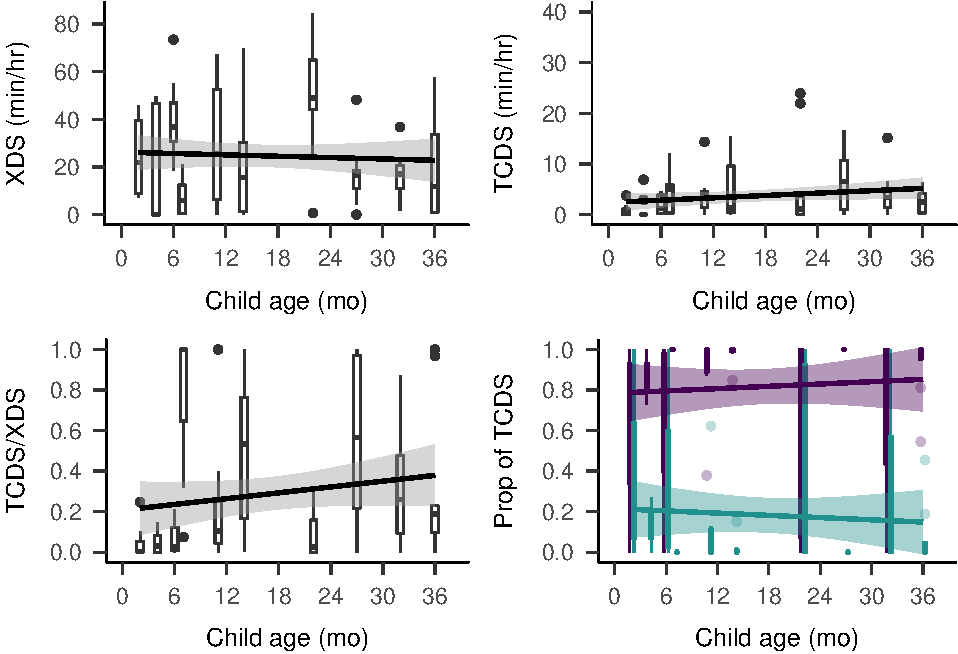
\includegraphics{Tseltal-CLE_files/figure-latex/plot_XDS_TDS_quantity_random-1.pdf}
\caption{}
\end{figure}

\begin{figure}
\centering
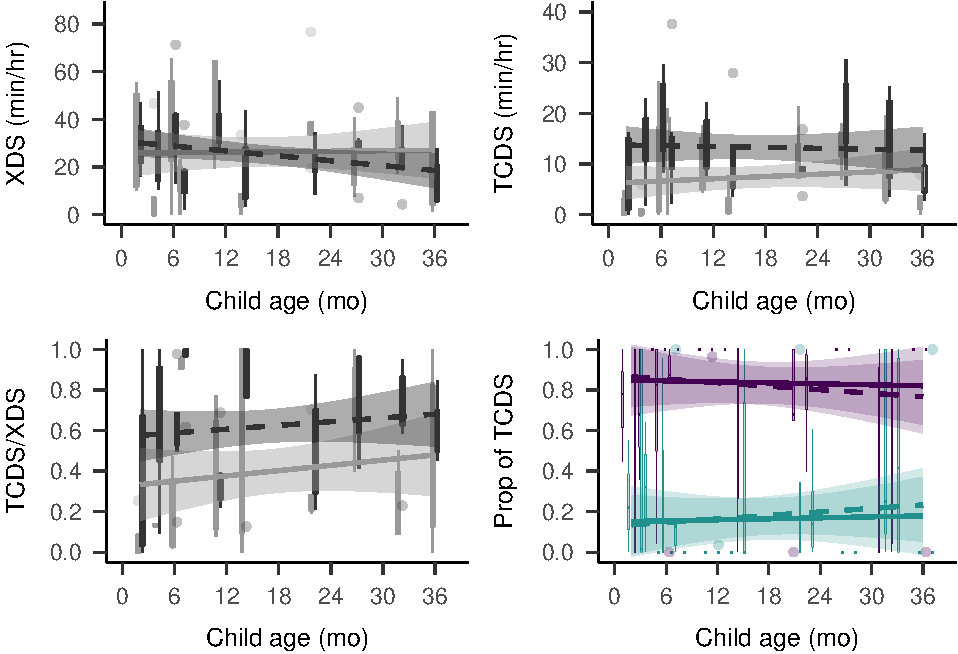
\includegraphics{Tseltal-CLE_files/figure-latex/plot_XDS_TDS_quantity_nonrandom-1.pdf}
\caption{}
\end{figure}

\begin{figure}
\centering
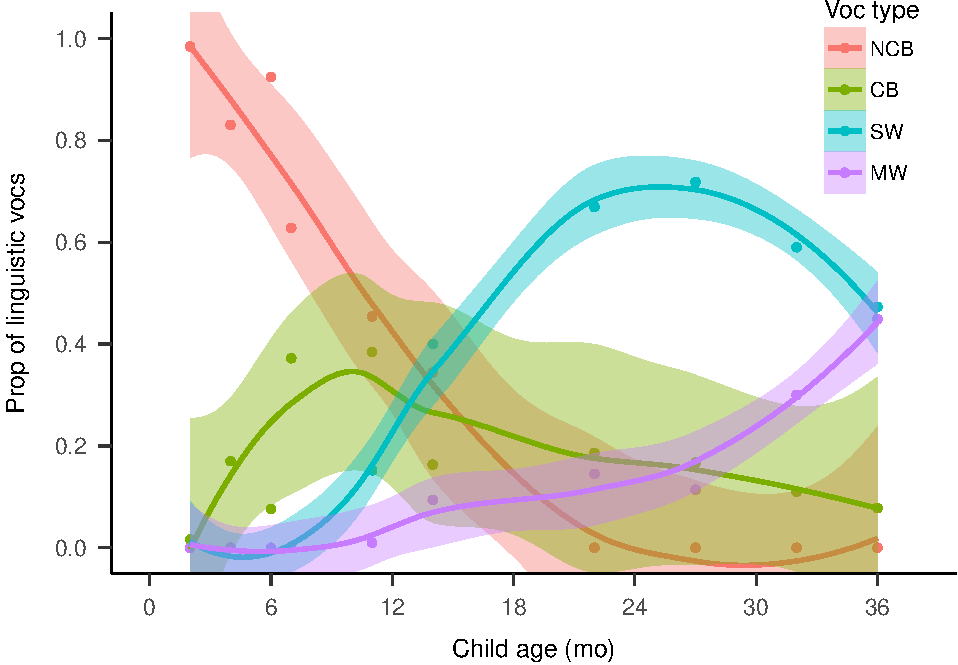
\includegraphics{Tseltal-CLE_files/figure-latex/plot_chi_voctypes_overall-1.pdf}
\caption{}
\end{figure}

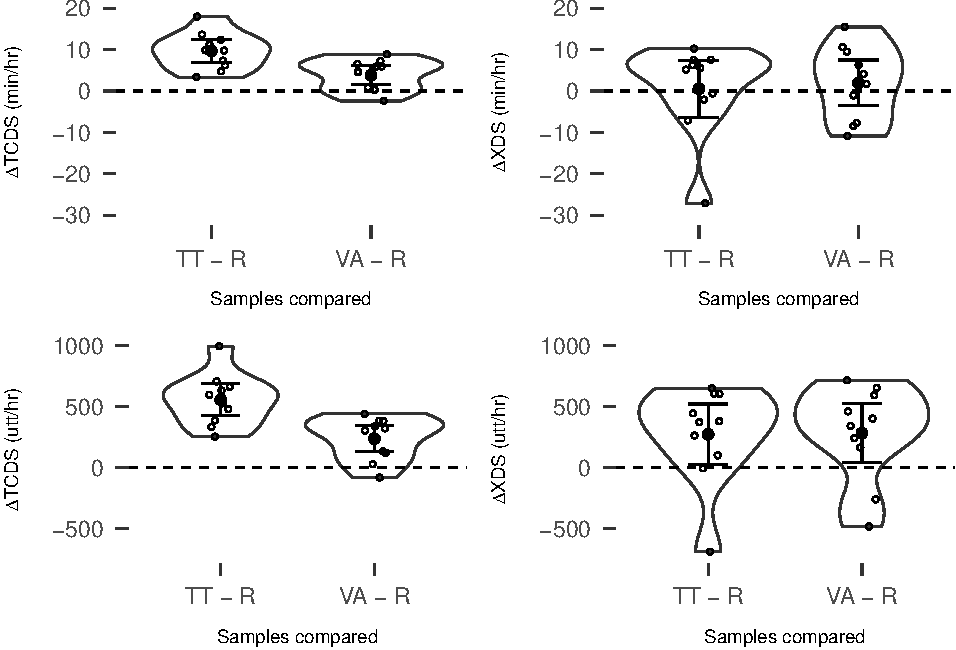
\includegraphics{Tseltal-CLE_files/figure-latex/plot_sample_differences-1.pdf}
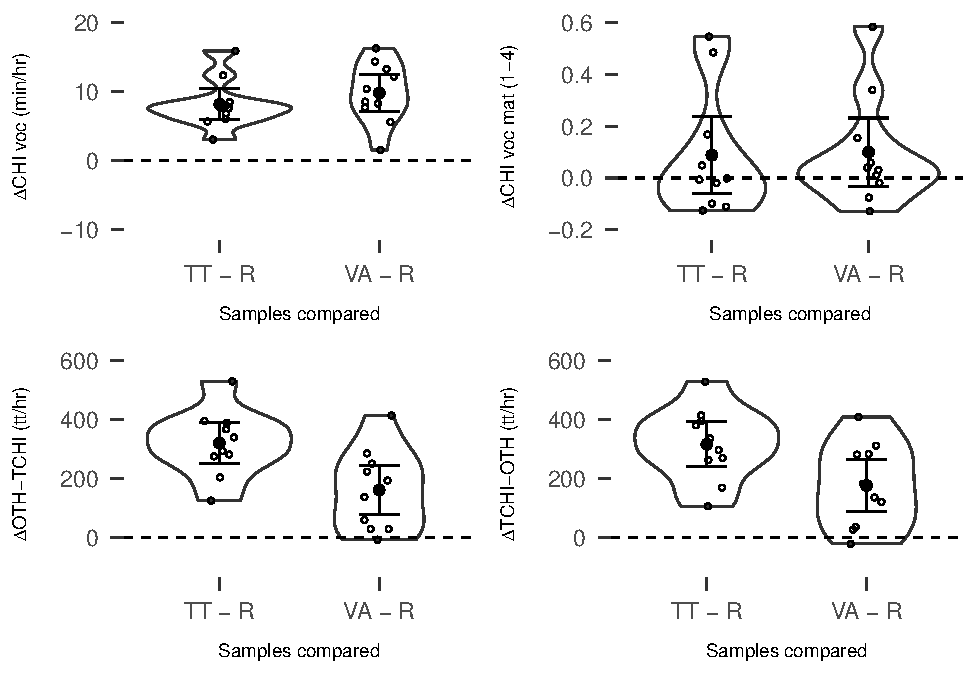
\includegraphics{Tseltal-CLE_files/figure-latex/plot_sample_differences-2.pdf}

\section{Discussion}\label{disc}

\subsection{Future directions}\label{disc-future}

\subsection{Conclusion}\label{disc-conclusion}

\section{Acknowledgements}\label{acknowledgements}

\newpage

\section{References}\label{refs}

\begingroup
\setlength{\parindent}{-0.5in} \setlength{\leftskip}{0.5in}

\hypertarget{refs}{}

\endgroup






\end{document}
